\documentclass{standalone}
\usepackage{tikz}
\usepackage{ctex,siunitx}
\usepackage{tkz-euclide}
\usepackage{amsmath}
\usetikzlibrary{patterns, calc}
\usetikzlibrary {decorations.pathmorphing, decorations.pathreplacing, decorations.shapes,}
\begin{document}
\small
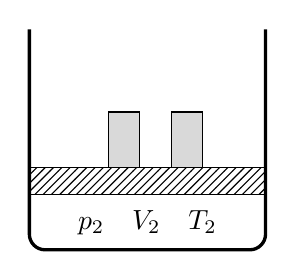
\begin{tikzpicture}[>=stealth,xscale=2,yscale=0.7]
  \draw [rounded corners=0.2cm, very thick](2,2)--(2,-2)--(3.5,-2)--(3.5,2);
  \draw [pattern=north east lines](2,-1) rectangle (3.5,-0.5);
  \draw [fill=gray!30](2.5,-.5) rectangle(2.7,.5);
  \draw [fill=gray!30](2.9,-.5) rectangle(3.1,.5);	
  \node at (5.5/2, -1.5){$p_2\quad V_2\quad T_2$};
\end{tikzpicture}
\end{document}